\documentclass[journal,a4paper]{IEEEtran}
\usepackage{fullpage}
\usepackage{float}
\usepackage[T1]{fontenc}

%\usepackage{color}
\usepackage{xcolor}
\usepackage{amsmath}
\usepackage{graphicx}
\usepackage{listings}

\begin{document}
\onecolumn

\title{COMP333: Assignment 2}
\author{James Ridey\\
44805632}
\maketitle
%
%\lstdefinestyle{customc}{
%  belowcaptionskip=1\baselineskip,
%  breaklines=true,
%  frame=L,
%  xleftmargin=\parindent,
%  language=,
%  showstringspaces=false,
%  basicstyle=\footnotesize\ttfamily,
%  keywordstyle=\bfseries\color{green!40!black},
%  commentstyle=\itshape\color{purple!40!black},
%  identifierstyle=\color{blue},
%  stringstyle=\color{orange},
%}

\definecolor{pblue}{rgb}{0.13,0.13,1}
\definecolor{pgreen}{rgb}{0,0.5,0}
\definecolor{pred}{rgb}{0.9,0,0}
\definecolor{pgrey}{rgb}{0.46,0.45,0.48}

\lstset{language=Java,
  showspaces=false,
  showtabs=false,
  tabsize=4,
  breaklines=true,
  showstringspaces=false,
  breakatwhitespace=true,
  commentstyle=\color{pgreen},
  keywordstyle=\color{pblue},
  stringstyle=\color{pred},
  basicstyle=\ttfamily,
  moredelim=[il][\textcolor{pgrey}]{$ $},
  moredelim=[is][\textcolor{pgrey}]{\%\%}{\%\%}
}

\pagenumbering{gobble}
\hyphenation{water question questions maximum}
\section*{Question 1}
\begin{enumerate}
	\item What this invarient is saying is that for every item in the queue, it is at least 1 distance away from the head of the queue. This holds true for eveyr iteration of the BFS algorithm because of a few reasons, the first is that nodes are added onto the end of the queue, the second is that we never visit the same node twice and the third reason is that BFS always expands equally in every direction. For these three reasons nodes in the queue will always be in ascending distance.
	\item For every visited node, the distance is made of a combination of the cells that are reachable (Fact 1) and the node that is the closest to them. BFS expands equally in all directions so every visited nodes distance is simply the closest previous node that used to be in the queue.
	\item 
\end{enumerate}

\section*{Question 2}
\begin{enumerate}
	\item For each loop of divideBasic we are subtracting b from a. For a worst case scenario this means we have something like 99999 / 1. Expressing this in the form a and b means we get $10^{L(a)}-1$ and $10^{L(b)-1}$. 

Given we are subtracting each loop iteration this means we have $\frac{10^{L(a)}-1}{10^{L(b)-1}}$ operations. And so the Big-Oh of divideBasic is 
	\begin{align*}
		&= \frac{10^{L(a)}-1}{10^{L(b)-1}} \\
		&= 10^{L(a)-(L(b)-1)} - 1 \\
		&= O(10^{L(a)-L(b)+1})
	\end{align*}
	\item A
	\item The best way to understand this question is with some graphs
	\\\\
	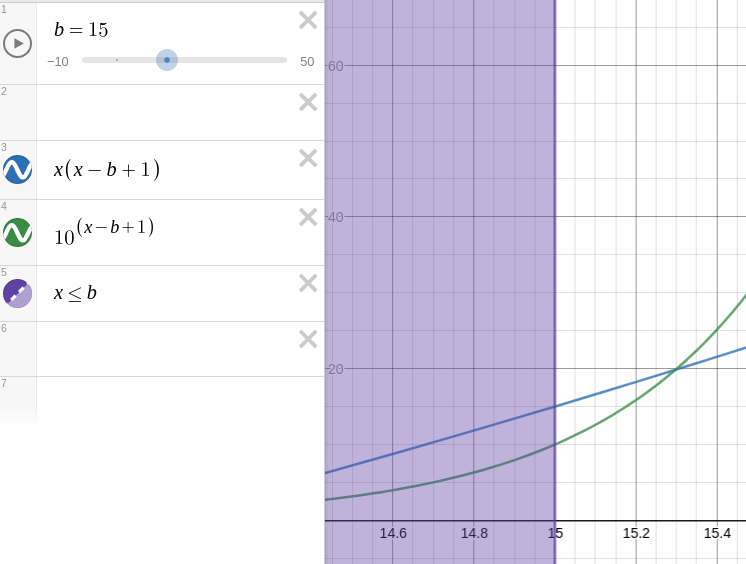
\includegraphics[scale=2]{divide-complexity-1} \\
	In this graph we have the green line as divideBasic and the blue line as divide, we have a L(b) of 15, L(a) being set as the x variable and y being O(n). From this graph we can see initially divideBasic wins out if the length of both numbers are the same, however it quickly loses out as the length of a grows.
	\\\\
	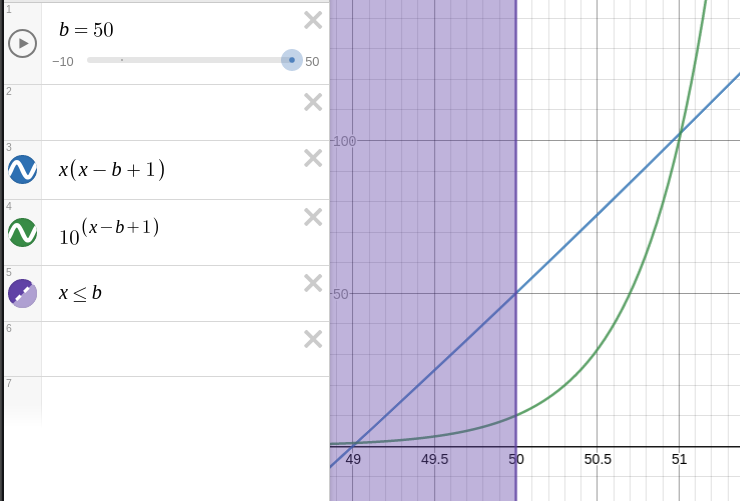
\includegraphics[scale=2]{divide-complexity-2} \\
	As b increases, divideBasic is the faster variant as long as a and b are the same length.
	\\\\
	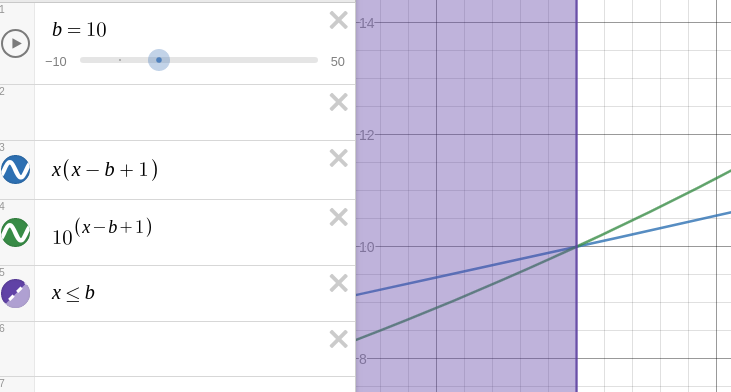
\includegraphics[scale=0.5]{divide-complexity-3} \\
	The exception to this rule is with lengths of b less than 10, this this case divide is always faster than divideBasic.
	\\\\
	In conclusion, divideBasic is only ever faster than divide when the lengths of the numbers are the same, for every other case divide wins out exponentially.	
\end{enumerate}

\section*{Question 3}
\begin{enumerate}
	\item A
	\item A
	\item A
\end{enumerate}

\section*{Question 4}
\begin{enumerate}
	\item Loop invariant: TODO
		  For this algorithm it runs until b is zero and for every iteration of the loop we divide b by 2. So this loop runs at least $log_2(b)$ times. During the loop operation we do 2 multiplications and 2 divisions, while 1 of the multiplications and 1 of the divisions is behind an if statement in the worse case scenario (Big-Oh), if a number was simply a 1 bit repeated it would always trigger the if statement.
		  
		  So for the worse case scenario we have
		  \begin{align*}
		  	&= log_2(b)(2mul + 2div) \\
		  	&= log_2(b)(2(L(a)L(b)) + 2(L(a)(L(a)-L(b)+1))) \\
		  	&= log_2(b)(2(L(a)(L(a)+1))) \\
		  \end{align*}
	\item A
	\item A
\end{enumerate}

\section*{Question 5}
- For the time complexity of Karatsuba we first need to find out how deep the tree of the recursion will go. Using what we understand of the algorithm and how it effectively splits the numbers in half each time. The depth of the tree is $log_2(max(L(a),L(b)))$.

Then for every node of the recursion we do the following
\begin{enumerate}
	\item Call Karatsuba another three times
	\item 2 additions
	\item 2 multiplications
	\item 2 subtractions
	\item 2 lessThanOrEqual's
	\item 2 modpows - (similar time complexity to modexp)	
\end{enumerate}

This effectively means we have the time complexity of
\begin{align*}
	&= log_2(max(L(a),L(b)))\cdot \left( 3(2add+2mul+2sub+2less+2modpow) \right) \\
	&= log_2(max(L(a),L(b)))\cdot \left( 3(2add+2mul+2sub+2less+2modpow) \right) \\
\end{align*}

- In what circumstance would you expect Karatsuba’s algorithm to be more efficient than the classical one?

\section*{Question 6}


\section*{Question 7}
Most of the RSA program is input parsing and checking to make sure that the input being passed is correct. Cutting out that, I've pasted below the meat of the program.
\begin{lstlisting}[language=Java]
public static void encrypt(Scanner scanner) {
	...
	
	BigInt p = randomprime(length, 32);
	BigInt q = randomprime(length, 32);
	BigInt n = p.multiply(q); //TODO: Replace with karatsuba
	BigInt totient = p.subtract(ONE).multiply(q.subtract(ONE));

	BigInt publicKey;
	while (true) {
		publicKey = randomprime(totient.toString().length(), 32);

		int a = Integer.valueOf(totient.toString());
		int b = Integer.valueOf(publicKey.toString());

		if (publicKey.lessOrEqual(totient) && egcd(a,b)[0] == 1) break;
	}

	int a = Integer.valueOf(publicKey.toString());
	int b = Integer.valueOf(totient.toString());
	int privateKey = minv(a,b);

	System.out.println("Public key: " + publicKey);
	System.out.println("Private key: " + privateKey);
	System.out.println("Modulus: " + n);

	System.out.print("Data to encrypt: ");
	s = scanner.nextLine();
	for (char c : s.toCharArray()) {
		int pki = Integer.valueOf(publicKey.toString());
		int pi = Integer.valueOf(p.toString());
		int qi = Integer.valueOf(q.toString());

		int zz = modexpv3(pi, qi, (int)c, pki);
		System.out.print(zz+" ");
	}
	System.out.println('\n');
}

public static void decrypt(Scanner scanner) {
	...
	
	System.out.print("Private key: ");
	String s = scanner.nextLine();
	BigInt privateKey = new BigInt(s);

	System.out.print("Modulus: ");
	s = scanner.nextLine();
	BigInt n = new BigInt(s);

	System.out.print("Data: ");
	s = scanner.nextLine();
	for (String v : s.split(" ")) {
		BigInt d = new BigInt(v);
		int c = Integer.parseInt(modexp(d, privateKey, n).toString());
		System.out.print((char)c);
	}
	System.out.println('\n');
}
\end{lstlisting}

For encryption, we need to generate a private key, a public key and a modulus. To do this we follow these steps
\begin{enumerate}
	\item Pick a random prime (p) and another random prime (q)
	\item Pick the public key to be a prime between 0 and the totient of p times q which for primes is $(p-1)\cdot (q-1)$.
	\item Check that the totient and the generated public key have a GCD of 1 and if not regenerate the public key.
	\item The private key is generated using the modular inverse of the public key and the totient.
	\item For every chuck in the data to be encrypted, take the modular exponent of the chunk, the public key and the modulus ($n = p\cdot q$)
\end{enumerate}

Decryption is a simpler process, for every chuck in the data to be decrypted, take the modular exponent of the chunk, the private key and the modulus and concatenate that all together.

\end{document}
